\documentclass[11pt]{article}
\usepackage{ucs}
\usepackage{graphicx}
\usepackage[utf8x]{inputenc} 
\usepackage[russian]{babel}  

\begin{document}
	\begin{enumerate}
	\item Дата собрания: 15.10.14
	\item Цель:
		\begin{itemize}
		\item Заменить омни-колеса на обычные
		\item Начать готовить профили для подъемника
		\end{itemize}
	\item Результаты:
		\begin{itemize}
		\item Было установлено два колеса, оба ведущие
		\item Профили были распилены на отдельные части определенного размера и пропилены отверстия для креплений
		\end{itemize}
	\item Идеи и планы:
		\begin{itemize}
		\item Установить оставшиеся колеса и испытать робота на поле
		\item Начать строить подъемник
		\end{itemize}
		\begin{figure} [h]
			\centering
			\begin{minipage}{0.3\linewidth}
				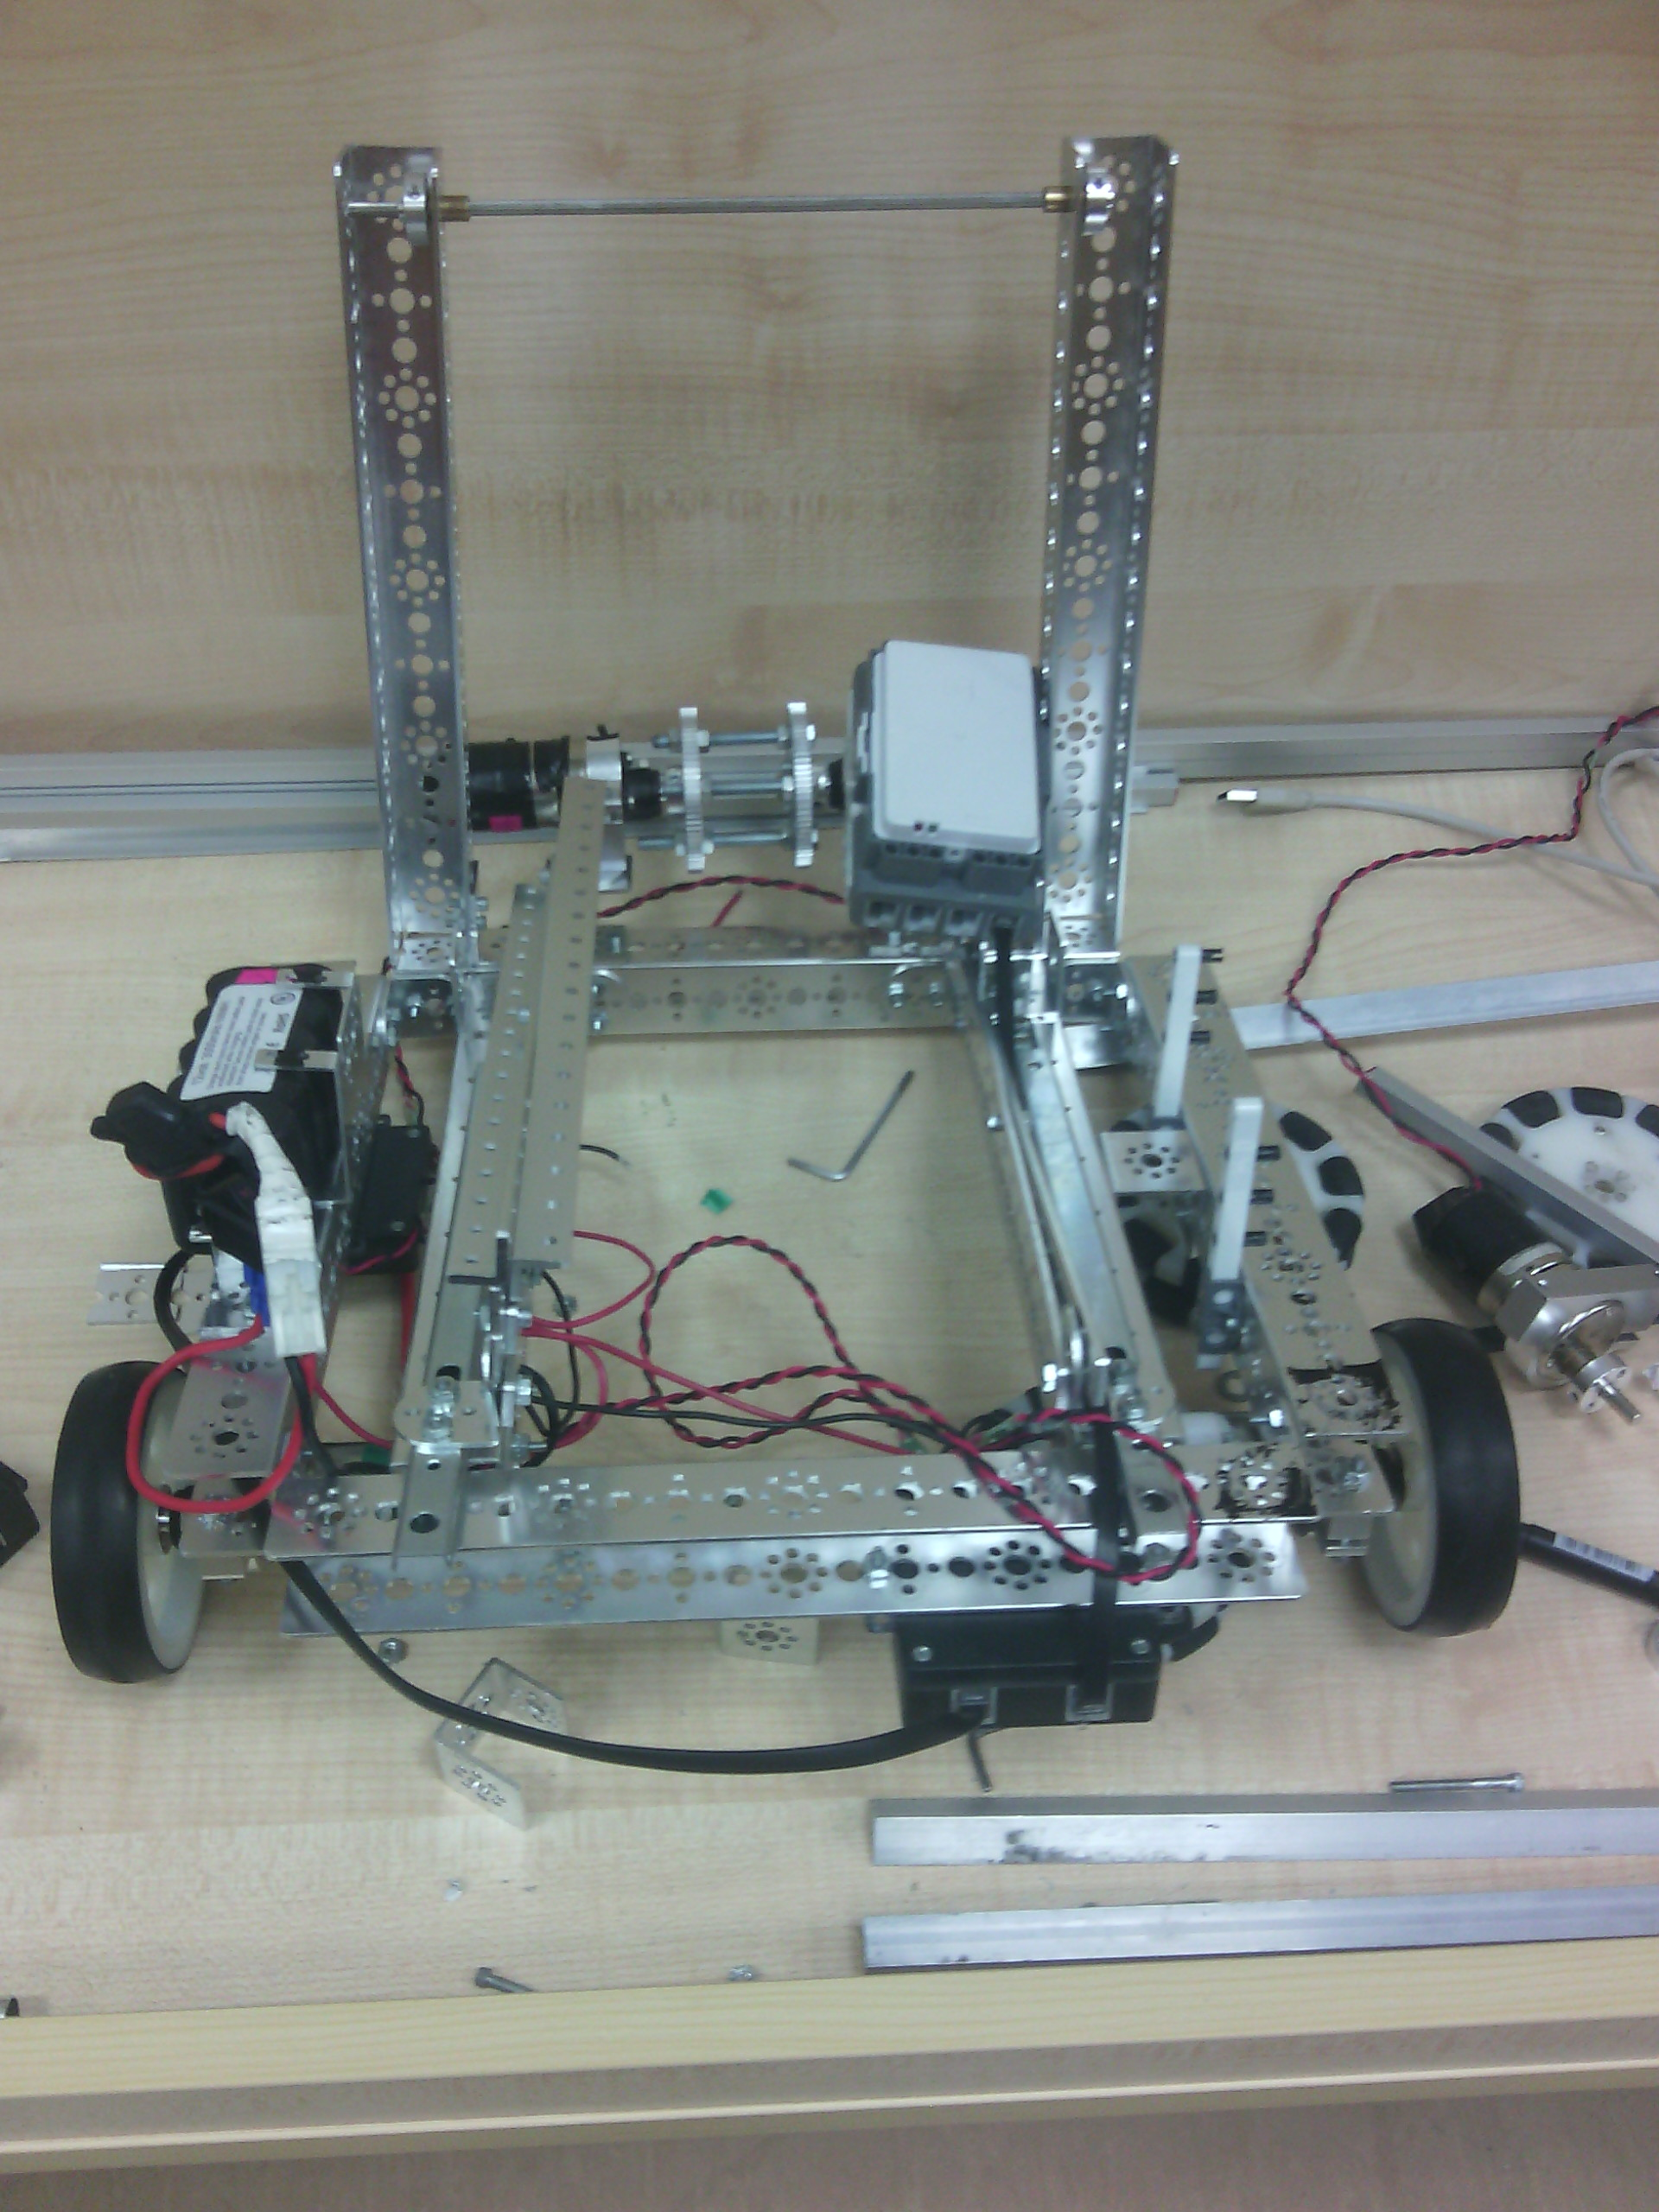
\includegraphics[width=35mm,height=35mm]{8_1_robot}\\ Рисунок 3
			\end{minipage}
		\end{figure}
	\end{enumerate}
\end{document}
	
